\chapter{Część przeglądowa}

\section{Przykładowa sekcja}


\subsection{Przykładowa subsekcja}
Quia ipsam non animi placeat amet sed. Cumque aut ratione velit expedita occaecati rerum qui. Cumque aut et quo repellat. Dolorem minima molestiae accusamus laboriosam qui. Neque quam qui natus optio quae. Przykładowy Refferal do obrazka nr \ref{fig:przykladowy-obrazek}.

\begin{figure}[ht]
        \centering
        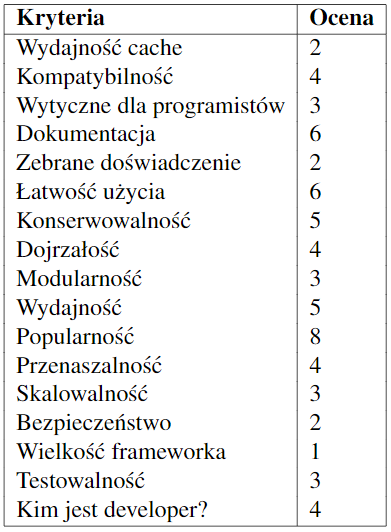
\includegraphics[width=16cm]{rysunek_1.png}
        \caption{Grafika przedstawiająca ocenę wpływu wybranego elementu na atrakcyjność danego narzędzia}
        \label{fig:rysunek_1}
\end{figure}

\newpage

\section{Druga sekcja}
Quia ipsam non animi placeat amet sed. Cumque aut ratione velit expedita occaecati rerum qui. Cumque aut et quo repellat. Dolorem minima molestiae accusamus laboriosam qui. Neque quam qui natus optio quae. Przykładowy Refferal do obrazka nr \ref{table:przykladowa-tabela}.

\begin{table}[htb]
	\centering
	\caption{Przykładowa tabela}
	\label{table:przykladowa-tabela}

    \begin{tabular}{| l | l |}
    \hline
    Nazwa komponentu & Licencja \\ \hline
    Graylog 2.5 & GNU General Public License v3 \\ \hline
    MongoDB 3.4 & GNU Affero General Public License v3 \\ \hline
    Elasticsearch 6.5.1 & Elastic License \cite{elastic-license} \\ \hline
    rsyslog 8.24.0 & GNU General Public License v3  \\ \hline
    NXLog CE 2.10.2150& NXLog Public License  \\ \hline
    Docker 18.09.1 & Apache License 2.0  \\
    \hline
    \end{tabular}
\end{table}

\newpage